% this is the non-them-dependent code for the Warner style file, based on Lankton theme
% Zach Warner, University of Wisconsin Madison, 12 December 2013
% contact: zwarner@wisc.edu

\documentclass[serif,mathserif,final]{beamer}
\usepackage{amsmath,amsfonts,amssymb,pxfonts,eulervm,xspace}
\usepackage{graphicx,tikz}
\usepackage{wrapfig}
\usepackage{textpos} 
\usepackage{ragged2e}
\usepackage[orientation=landscape,size=custom,width=48,height=36,scale=.6,debug]{beamerposter}


%-Getting your school colors involved-----------------
\definecolor{wiscored}{RGB}{183,1,1} % Wisco red, from http://www.uc.wisc.edu/brand/web/colors.php. I find it easiest to use a web source to translate hex to rgb. Most schools have both available, though.
\definecolor{wiscogold}{RGB}{231, 217, 193} % in case you want to use the Wisconsin gold. I don't think it shows up nicely with the white, red, and black, though.

%-Go find your crest and logo------------------------
% I found Wisconsin's here: http://www.uc.wisc.edu/brand/templates-and-downloads/web-logos.php

% Usually you want the one with the colors reversed for the header, since you're using the primary color as the banner. Also, I highly recommend using a pdf editor (preview will work fine) to crop the logo down to size so that you can fit it in the banner.

% Generally, only use pdf output for graphics on your poster. Never png, jpeg, jpg, etc. You don't want pixelated images.

%-Defining colors and fonts-----------------
\mode<all>
\setbeamercolor{headline}{bg=wiscored}
\setbeamercolor{footline}{bg=wiscored}
\setbeamerfont{footline}{size=\large}
\setbeamercolor{separation line}{bg=wiscored}
\setbeamercolor{title in headline}{fg=white}
\setbeamercolor{author in headline}{fg=white}
\setbeamercolor{institute in headline}{fg=white}

\setbeamercolor{framesubtitle}{fg=white, bg=wiscored}
\setbeamercolor{author in head/foot}{fg=white,bg=wiscored}
\setbeamercolor{title in head/foot}{fg=white,bg=wiscored}
\setbeamercolor{website in footline}{fg=white,bg=wiscored}
\setbeamercolor{email in footline}{fg=white,bg=wiscored}

\setbeamercolor*{normal text}{fg=black, bg=white}
\setbeamercolor*{block body}{fg=black,bg=white}
\setbeamercolor*{block title}{fg=white,bg=wiscored}
\setbeamerfont{block title}{size=\normalsize,series=\sc}
\setbeamercolor{upper separation line head}{fg=black}
\useinnertheme{circles}
\setbeamertemplate{itemize}[circle]
\newenvironment{circenv}{\only{\setbeamercolor{local structure}{fg=black}}}{} %this makes it so that itemized lists have black circles, in keeping with our color theme, rather than blue trianges.

\setbeamertemplate{navigation symbols}{}  %  turn the navigation symbols off for a poster

%-Setting the template for each block of text-----------------------
\setbeamertemplate{block begin}{
  \vskip.5ex
  \begin{beamercolorbox}[leftskip=1ex,colsep*=.5ex]{block title}%
    \usebeamerfont*{block title}{\Large \insertblocktitle}
    \vskip.5ex
  \end{beamercolorbox}%
  {\ifbeamercolorempty[bg]{block body}{}{\nointerlineskip\vskip-0.5pt}}%
  \usebeamerfont{block body}%
  \begin{beamercolorbox}[colsep*=.5ex,sep=.5ex,vmode]{block body}%
  \justifying
    \ifbeamercolorempty[bg]{block body}{\vskip-.25ex}{\vskip-.5ex}\vbox{}%
  }
  \setbeamertemplate{block end}{
  \end{beamercolorbox}
}

%-Setting the headline template--------------------------------
\setbeamertemplate{headline}{
  \leavevmode

  \begin{beamercolorbox}[wd=\paperwidth]{headline}
    \begin{columns}[T]
      \begin{column}{.491\paperwidth}
        \vskip6ex %use vskip to achieve the vertical centering you want based on logo and font sizes
        \raggedleft
        \usebeamercolor{title in headline}{\color{fg}\textbf{\huge{\inserttitle}}\\[1ex]}
        \usebeamercolor{author in headline}{\color{fg}\huge{\insertauthor}\\[1ex]}
        \usebeamercolor{datein headline}{\color{fg}\Large{\insertdate}\\[1ex]}        
        \usebeamercolor{institute in headline}{\color{fg}\Large{\insertinstitute}\\[1ex]}
        \vskip2ex
      \end{column}
      \begin{column}{.005\paperwidth}
      \end{column}
      \begin{column}{.504\paperwidth}
        \vskip6ex
       \raggedright
        
\includegraphics[height=0.1\paperwidth]{uwlogo.pdf}
        \vspace{1pt}
      \end{column}
    \end{columns}
  \end{beamercolorbox}

  \begin{beamercolorbox}[wd=\paperwidth]{lower separation line head}
    \rule{0pt}{2pt}
  \end{beamercolorbox}
}

%-Setting the footline template-------------------------------
\setbeamertemplate{footline}{
  \begin{beamercolorbox}[wd=\paperwidth]{upper separation line foot}
    \rule{0pt}{2pt}
  \end{beamercolorbox}
  \leavevmode%
  \begin{beamercolorbox}[ht=4ex,leftskip=1cm,rightskip=1cm]{author in head/foot}%
  \begin{columns}
    \begin{column}{.43\paperwidth}
    \hspace{1cm}
    \usebeamercolor{website in footline}{\color{fg} \footleft}
    \end{column}
    \begin{column}{.14\paperwidth}
    \centering
     \usebeamercolor{date in footline}{\color{fg} \footmid}
     \end{column}
     \begin{column}{.43\paperwidth}
     \hfill
    \usebeamercolor{email in footline}{\color{fg} \footright}
    \hspace{1cm}
    \end{column}
    \end{columns}
    \vskip1ex
  \end{beamercolorbox}
  \vskip0pt%
  \begin{beamercolorbox}[wd=\paperwidth]{lower separation line foot}
    \rule{0pt}{2pt}
  \end{beamercolorbox}
}



%-- Header and footer information ----------------------------------
\newcommand{\footleft}{PolMeth Annual Conference 2013}
\newcommand{\footright}{zwarner@wisc.edu}
\newcommand{\footmid}{\today}
\title{A Wisconsin Poster Template}
\author{Zach Warner}
\date{\today}
\institute{zwarner@wisc.edu} % well, that's a lie. But email makes more sense here
%-------------------------------------------------------------------


%-- Main Document --------------------------------------------------
\begin{document}
\begin{frame}{}
  \begin{columns}[t]

    %-- Column 1 ---------------------------------------------------
    \begin{column}{0.32\linewidth}

      %-- Block 1-1
      \begin{block}{Abstract}
        Some text. Don't worry, the white space above the first texts blocks will disappear as the columns fill up.
      \end{block}

      %-- Block 1-2
       \begin{block}{Motivation}      
       A great place for some ponderous questions, and perhaps a model or two. If using a model, it might get shortened due to the columns. I'd use \texttt{multiline} to make it work. 
      \end{block}



     %-- Block 1-3
     \begin{block}{A Test}
         Run it.
         \begin{itemize}
          \item<circ@1->
          This code makes sure the colors of the circles match the color theme.
           \item<circ@1->
           If you change this to fit your school, you can set \texttt{fg=black} to whatever rgb coordinates you desire.
            \item<circ@1->
            While I'm in this list, note that the normal line break of won't work here. 
			\item<circ@1->            
            Instead, use \texttt{par}, a tilde, and another \texttt{par}.
         \end{itemize}
         One final snafu: the crest won't be where it should be whenever you compile for the first time. Always compile twice when you make adjustments to it.
     \end{block}
     
     
    \end{column}%1

    %-- Column 2 ---------------------------------------------------
    \begin{column}{0.32\linewidth}

      %-- Block 2-2
      \begin{block}{Results}
      Put your main results, particularly attractive visual displays, here.
       \begin{figure}[htb]
 % \vspace{-5pt} usually a figure will leave too much white space, so use negative vspace to adjust it to your taste
  \centering
          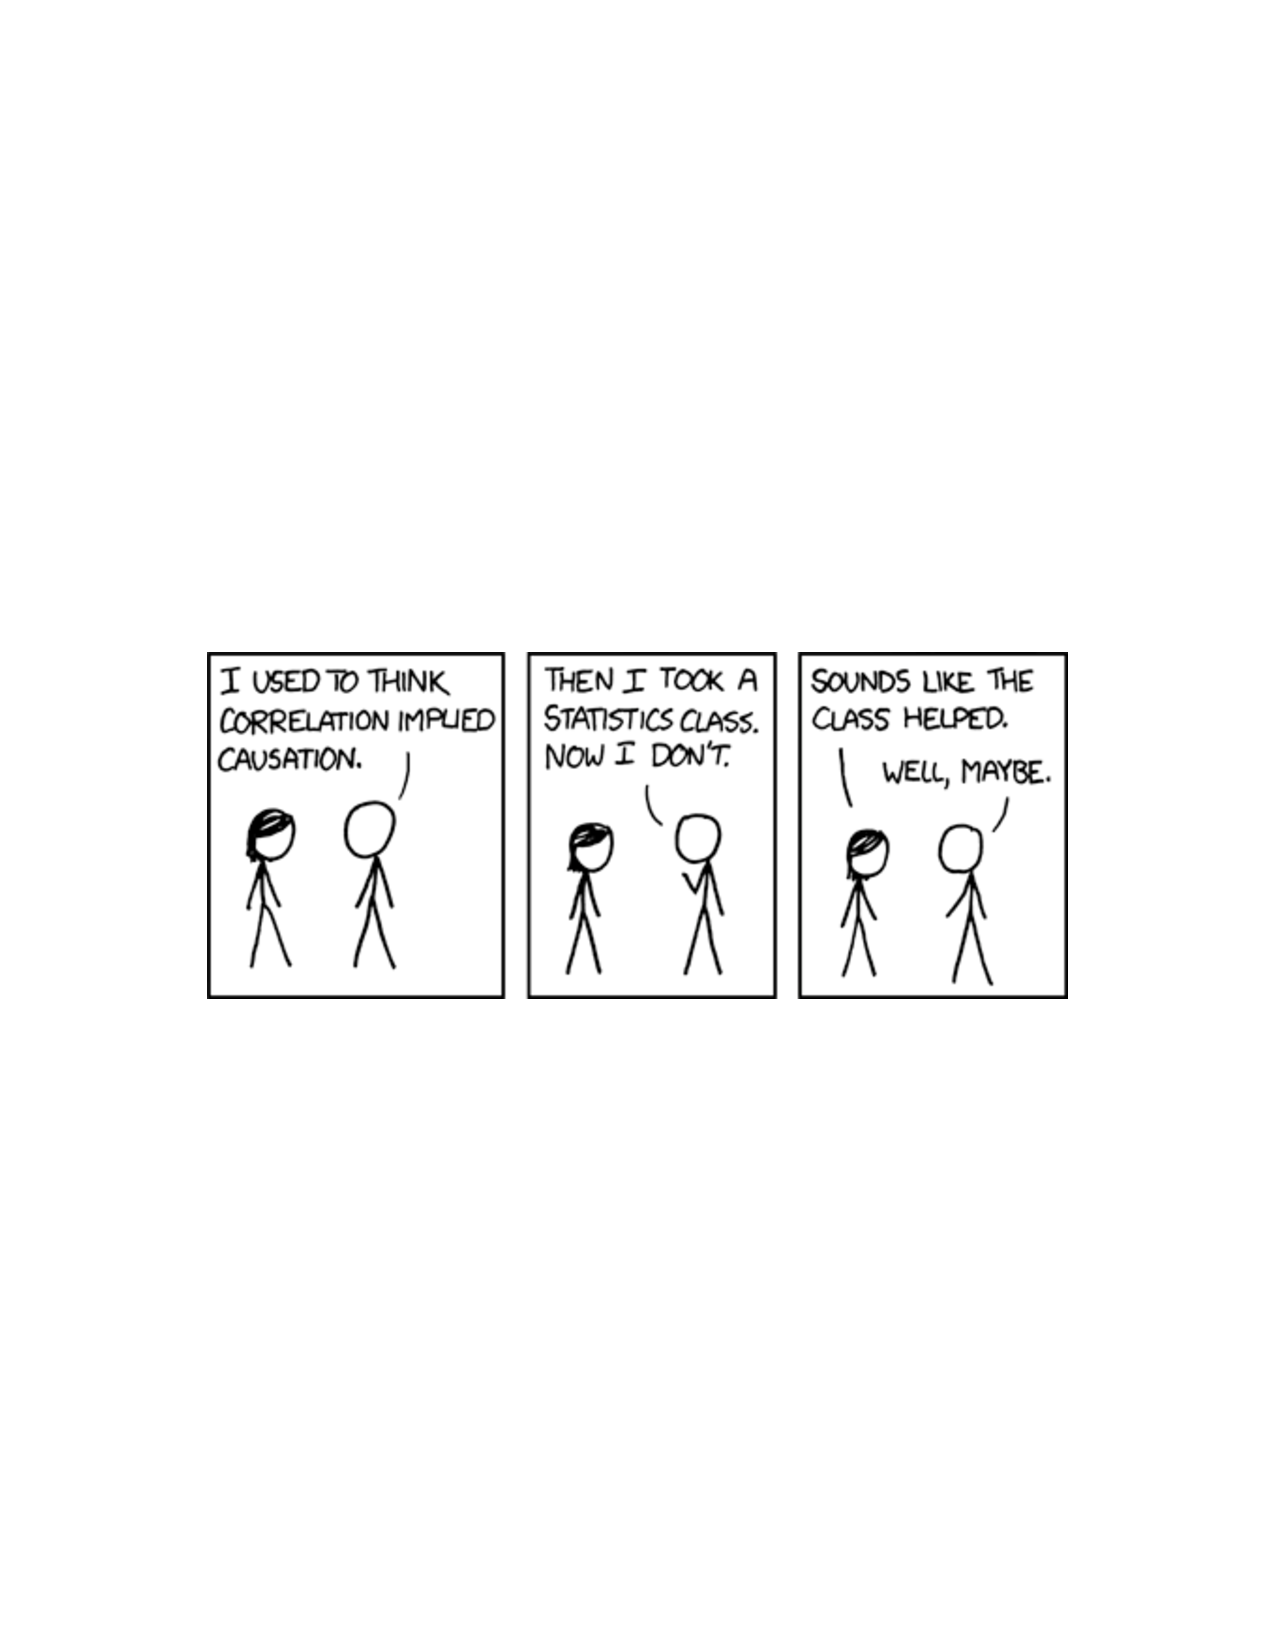
\includegraphics[width=\columnwidth]{correlation.pdf}
        \end{figure}
        Source: \texttt{http://xkcd.com/552/}.
      \end{block}

  %-- Block 2-3
      \begin{block}{Robustness}
They don't think it be like it is, but it do.
      \end{block}    

    \end{column}%2

    %-- Column 3 ---------------------------------------------------
    \begin{column}{0.32\linewidth}

      %-- Block 3-1
      \begin{block}{Extensions 1}
  This is a great place to insert tables and graphics side-by-side using \texttt{column} or \texttt{wrapfig}. Make sure you use \texttt{booktabs} for tables to make them prettier.
      \end{block}

      %-- Block 3-2
      \begin{block}{Extensions 2}
      One last figure, possibly just to show some interesting avenues for future research. 
      \end{block}

	%-- Block 3-3
	 \begin{block}{Conclusion}
	Based on the template ``Lankton'' by Shawn Lankton, available at \texttt{http://		www.shawnlankton.com/2008/06/latex-beamer- \\ poster-theme-and-template/}. \par ~ \par
Feel free to email me questions, comments, hatemail, or thanks, if so inclined.
      \end{block}

    \end{column}

  \end{columns}
  
%--- The crest----------------------------------------------------
  \begin{tikzpicture}[remember picture,overlay] 
            \node[opacity=.1, at=(current page.south west),anchor=south west,inner sep=-160pt] {
                
\includegraphics[width=.5\paperheight]{uwcrest.pdf}
            };
        \end{tikzpicture}
        % higher numbers for opacity mean a brighter picture, but this can make text harder to read
        % the anchor is the bottom left column, inner sep moves it so it bleeds off the page.
        % adjust inner sep according to taste
        
        %note that the first time you compile, the crest won't be where you want it to be. Compile a second time and it should be fine.
        
\end{frame}
\end{document}
